\documentclass[a4paper,12pt]{article}
\usepackage{amsmath}
\usepackage{amssymb}
\usepackage[polish]{babel}
\usepackage{polski}
\usepackage[utf8]{inputenc}
\usepackage{indentfirst}
\usepackage{geometry}
\usepackage{array}
\usepackage[pdftex]{color,graphicx}
\usepackage{subfigure}
\usepackage{afterpage}
\usepackage{setspace}
\usepackage{color}
\usepackage{wrapfig}
\usepackage{listings}
\usepackage{datetime}

\renewcommand{\onehalfspacing}{\setstretch{1.6}}

\geometry{tmargin=2.5cm,bmargin=2.5cm,lmargin=2.5cm,rmargin=2.5cm}
\setlength{\parindent}{1cm}
\setlength{\parskip}{0mm}

\newenvironment{lista}{
\begin{itemize}
  \setlength{\itemsep}{1pt}
  \setlength{\parskip}{0pt}
  \setlength{\parsep}{0pt}
}{\end{itemize}}

\newcommand{\linia}{\rule{\linewidth}{0.4mm}}

\definecolor{lbcolor}{rgb}{0.95,0.95,0.95}
\lstset{
    backgroundcolor=\color{lbcolor},
    tabsize=4,
  language=C++,
  captionpos=b,
  tabsize=3,
  frame=lines,
  numbers=left,
  numberstyle=\tiny,
  numbersep=5pt,
  breaklines=true,
  showstringspaces=false,
  basicstyle=\footnotesize,
  identifierstyle=\color{magenta},
  keywordstyle=\color[rgb]{0,0,1},
  commentstyle=\color{blue},
  stringstyle=\color{red}
  }

\begin{document}

\noindent
\begin{tabular}{|c|p{11cm}|c|} \hline 
Grupa 4 & Barbara Nowak, Piotr Tomaszewski & \ddmmyyyydate\formatdate{25}{11}{2016} \tabularnewline
\hline 
\end{tabular}


\section*{Zadanie 3 - Mnożenie macierzy CUDA}

Celem naszego zadania było obliczenie iloczynu dwóch macierzy kwadratowych ale z użyciem karty graficznej i technologii CUDA.


Program uruchamiany jest z argumentem: \quotedblbase rozmiarMac \textquotedblright - to rozmiar macierzy. Pierwszym etapem jest sprawdzenie poprawności podanego rozmiaru macierzy. Początkowo zaimplementowaliśmy funkcję gpuErrchk(), która sprawdza poprawnosc dzialania GPU i w razie ewentualnych problemów wypisuje adekwatny komunikat z kodem błędu. Następnie podobnie jak w zadaniu 1, deklarujemy potrzebne zmienne oraz macierze.  Już w pierwszym etapie zauważamy, że  CUDA posiada własny typ do deklaracji zmiennych czasowych.
Ważną rzeczą w CUDA jest alokowanie pamięci na karcie graficznej za pomocą funkcji cudaMalloc():

\begin{lstlisting}
	gpuErrchk(cudaMalloc((void**) &d_A, sizeof(float)*rozmiarMac*rozmiarMac));
	gpuErrchk(cudaMalloc((void**) &d_B, sizeof(float)*rozmiarMac*rozmiarMac));
	gpuErrchk(cudaMalloc((void**) &d_C, sizeof(float)*rozmiarMac*rozmiarMac));
\end{lstlisting}

Deklarując rozmiar grida oraz ilość wątków w bloku, korzystamy ze specjalnej zmiennej typu dim3, która reprezentuje krotkę 3-wymiarową, jakiej używamy do określenia liczby uruchomionych bloków, choć tak naprawdę tworzymy siatkę 2-wymiarową. Ostatni (trzeci) element instrukcji posiada domyślną wartość 1, dzięki czemu program działa poprawnie).
\begin{lstlisting}
	dim3 grids(rozmiarGrid, rozmiarGrid); 
	dim3 blocks(rozmiarBlok, rozmiarBlok); 
\end{lstlisting}
Wywołując funkcję uzupełniającą macierze, musimy pamiętać aby zmienne typu dim3 przekazać do systemu wykonawczego <<<grids, blocks>>> a następnie zablokować bieżący wątek aplikacji do czasu zakończenia wszystkich oczekiwanych obliczeń na karcie graficznej.
\begin{lstlisting}
	uzupelnij <<<grids, blocks>>> (rozmiarMac, d_A, d_B);
	cudaDeviceSynchronize();
\end{lstlisting}

Podobnie jak w poprzednich zadaniach musimy przystąpić do zmierzenia czasu wykonywanych obliczeń, tutaj CUDA również posiada własne wbudowane funkcje. Etapy: uruchamiamy pomiar czasu; wywołujemy funkcję odpowiedzialną za obliczenia; ponownie blokujemy bieżący wątek aplikacji do czasu zakończenia wszystkich oczekiwanych obliczeń na karcie graficznej; zatrzymujemy licznik czasu. Po zakończeniu pomiarów musimy skopiować dane między karta graficzną a pamiecia RAM, do czego zastosujemy funkcję cudaMemcpy, gdzie kolejne parametry to odpowiednio: wskaźnik na obszar pamięci, do której nastąpi kopiowanie, wskaźnik na obszar pamięci, z której nastąpi kopiowanie, liczba bajtów do skopiowania oraz wybór kierunku kopiowania - w tym przypadku kopiujemy z karty graficznej do pamięci RAM komputera.
\begin{lstlisting}
	cudaEventRecord(czasStart, 0);
	obliczC <<<grids, blocks>>> (rozmiarMac, d_A, d_B, d_C); // 
	cudaDeviceSynchronize(); 
	cudaEventRecord(czasStop, 0);
	cudaEventSynchronize(czasStop); 
	
	gpuErrchk(cudaMemcpy(C, d_C , sizeof(float)*rozmiarMac*rozmiarMac, cudaMemcpyDeviceToHost));
\end{lstlisting}
Ostatnim krokiem jest zwolnienie wcześniej zaalokowanej pamięci na karcie graficznej oraz obliczenie czasu wykonywanych obliczeń za pomocą funkcji cudaEventElapsedTime.
\begin{lstlisting}
	cudaFree(d_A);
	cudaFree(d_B);
	cudaFree(d_C);	
	free(C); 	
	gpuErrchk(cudaEventElapsedTime(&roznica, czasStart, czasStop));
\end{lstlisting}
\begin{wrapfigure}{r}{0.5\textwidth}
	\vspace{-40pt}
	\begin{center}
		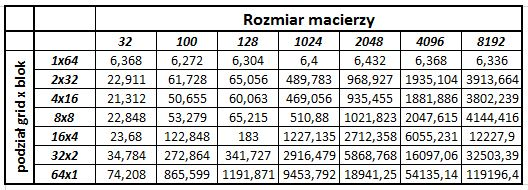
\includegraphics[width=0.5\textwidth]{zdj1.jpg}
	\end{center}
	\vspace{-20pt}
	\caption{Tabela zależności czasów od rozmiaru macierzy i gridu x bloku.}
	\vspace{25pt}
\end{wrapfigure}

Tabela obok przedstawia czasy [ms] w zależności od rozmiaru macierzy i rozmiaru bloku gridu. Dla rozmiaru grid x blok [1x64] czasy są porównywalne, nie zależnie jaki rozmiar macierzy byśmy zastosowali. Jednak przy zmianach w podziale i wzroście rozmiaru macierzy czasy znacznie wzrastają. Może nie jest to wzrost paraboliczny, jednak widać znaczny przyrost czasu między podziałami [8x8] a [16x4].


\begin{wrapfigure}{r}{0.5\textwidth}
	\vspace{-40pt}
	\begin{center}
		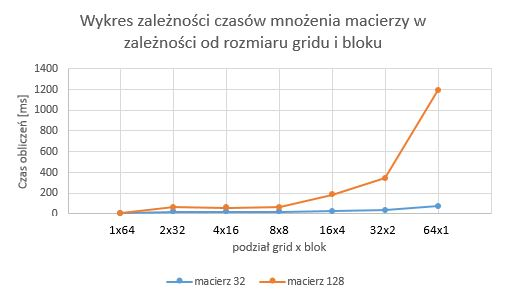
\includegraphics[width=0.5\textwidth]{zdj2.jpg}
	\end{center}
	\vspace{-20pt}
	\caption{Wykres porównania czasów 2 macierzy.}
	\vspace{35pt}
\end{wrapfigure}


Wykres przedstawia czas obliczeń dwóch wybranych rozmiarów macierzy na procesorze graficznym w zależności od podziału bloku i gridu. Tutaj potwierdzają się słowa które napisaliśmy powyżej, że dla podziału [16x4] czas obliczeń się wydłuża. Im większy rozmiar macierzy, tym czas będzie jeszcze większy. Jeślibyśmy narysowali wykresy z wszystkimi rozmiarami macierzy, to zauważylibyśmy, że macierze o podobnych rozmiarach mają podobne czasy, co w porównaniu z wielkimi rozmiarami powoduje nałożenie na siebie linii wykresu sprawiając, że wykres jest mało czytelny.

\textbf{Podsumowanie:} 
Podczas wykonywania zadania przy projekcie napotkaliśmy się na problem związany z odczytywaniem błędów. Bywało, że czasy wykonywania wychodziły 0 ms. Na początku problem wyniknął z niepoprawnej konwersji typów zmiennych. Później problem pojawił się przy odczytywaniu macierzy o dużych rozmiarach. Okazało się, że typ double zajmuje zbyt dużo pamięci, czego wynikiem był błąd. Zmieniliśmy typy macierzy z double na float i wyniki zaczęły wychodzić poprawne. Warto zabezpieczyć kod poprzez odczytywanie błędów powstałych w karcie graficznej, ponieważ dzięki temu mogliśmy zobaczyć co tak naprawdę jest nie tak.

\end{document}
